\documentclass{article}
\usepackage[spanish]{babel}
	\deactivatetilden
\spanishdecimal{.}
\addto\captionsspanish{\def\tablename{Tabla}}
\addto\captionsspanish{\def\listtablename{\'Indice de tablas}}
\usepackage[numbers,sort&compress]{natbib}
\usepackage[T1]{fontenc}
\usepackage[utf8]{inputenc}
\usepackage{graphicx}
\usepackage{url}
\usepackage{graphicx}
\graphicspath{{Figuras/}}
\usepackage[numbers,sort&compress]{natbib}
\usepackage[clearempty,pagestyles]{titlesec}
\usepackage{anysize}
\usepackage{xcolor, colortbl}
\usepackage{array, multirow, multicol}
\usepackage{enumerate} 

\def\baselinestretch{1.5}
\papersize{27.9cm}{21.5cm} 
\marginsize{2cm}{2cm}{1cm}{1cm}

\title {Red Neuronal}
\author{Julio Garc\'ia}
\pagestyle{empty}

\pagestyle{empty}
\begin{document}
	\renewcommand{\listtablename}{Índice de tablas}
	\renewcommand{\tablename}{Cuadro}
	\maketitle
	
	\section{Introducción}
	El estudio de variables y la relación de los efectos e interacciones entre ellas cambiando sus valores, es de suma importancia para la vida real. En la realidad, los diseños de experimentos se presentan en diversas áreas, como la medicina, biología, física experimental, psicología, negocios, entre otras. Dicho estudio, se vuelve indispensable para poder establecer relaciones o hipótesis que se desean probar.\\
	Una de las industrias que actualmente está creciendo exponencialmente, es el reconocimiento de imágenes, debido a que diferentes empresas están recurriendo a tecnología basada en algoritmos de reconocimiento para poder identificar alguna variable estudiar. Un caso de estudio es el reconocimiento facial de una persona a través de una fotografía, dichos reconocimiento se basan en algoritmos como las redes neuronales. En el presente trabajo se busca como objetivo evaluar el impacto que tienen las diferentes probabilidades de coloreo en el desempeño de una red neuronal de identificación de dígitos. 

	
	\section{Desarrollo}
	En este trabajo se estudia el impacto que tiene el valor de probabilidades de colores en dígitos con respecto al desempeño de una red neuronal. Dicho coloreo se divide en tres colores: negro, gris y blanco, la probabilidad de coloreo de cada color se va a tomar como cada uno de los factores en un diseño factorial.\\


	\section{Experimentación y resultados}
	En esta sección se describe el ambiente computacional y los resultados obtenidos con la simulación. El código de dicha simulación fue realizado en el lenguaje computacional Python en una computadora personal con procesador 1 Intel Core i7, con memoria RAM de 16GB y hasta 8 núcleos de procesamiento. Dicho código fue incorporado en el repositorio \cite{p_a}. Se tomó como base el código de Elisa Schaeffer \cite{pa}, en el que se realizaron las variaciones requeridas. El código base para la realización del diseño factorial fue tomado de \cite{pa2} y se realizó en lenguaje R.\\ 
    \begin{enumerate}
    \item El puntaje de la red neuronal está basado en la cantidad de aciertos, es decir, las veces que identificó correctamente cada uno de los dígitos correspondientes. Dicho valor se encuentra en la diagonal principal de la matriz que contiene los contadores. Para este trabajo. Nuestra función F es igual a la cantidad de total de aciertos entre el total de dígitos en la imagen.  
    \item Es importante mencionar lo siguiente: se decidió discretizar (categorizar) los valores de las variables a estudiar, lo anterior debido a que se tiene  un conocimiento a priori de que valores se pueden tomar y presentar un mejor comportamiento esperado. Se realizaron corridas con diferentes niveles en las probabilidades de coloreo para negro, gris y blanco, los valores de dichos niveles son: $\{ 0.30, 0.60. 0.90 \}$. Estos niveles fueron seleccionados de forma en que se distribuyeran a lo largo del intervalo ($0:1$).
    \item 	Se decidió correr cada combinación de probabilidades tres veces, por lo cual, la cantidad de replicas son tres por experimento.  Por lo anterior, podemos decir que el diseño factorial es de tres factores con tres niveles y tres replicas en cada uno de ellos.
    \end{enumerate}
	  
	La gráfica que representa el efecto que tiene la probabilidad de coloreo de cada color es la siguiente:  
	    	
	    	\begin{figure}[h!]
	    	\centering
	    	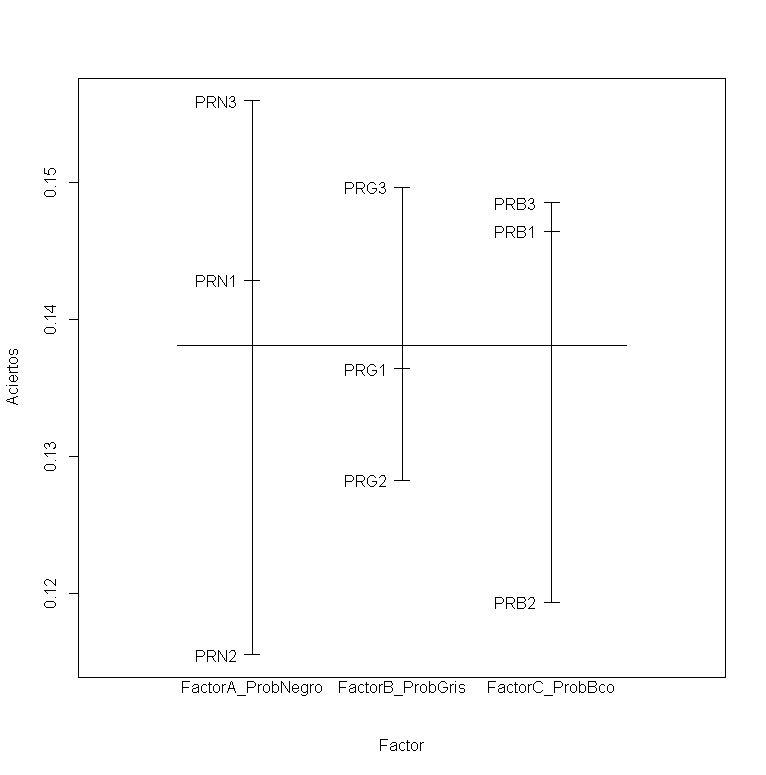
\includegraphics[width=0.7\linewidth]{Rplot02.png}
	    	\caption{Gráfica de efectos principales.}
	    	\label{fig:imagen1}
	    	\end{figure}
    
    % Table generated by Excel2LaTeX from sheet 'Hoja1'
    \begin{table}[htbp]
    	\centering
    	\caption{ANOVA}
    	\begin{tabular}{lrrrrrr}
    		& \multicolumn{1}{l}{Df} & \multicolumn{1}{l}{Sum Sq} & \multicolumn{1}{l}{Mean   Sq} & \multicolumn{1}{l}{F value} & \multicolumn{1}{l}{Pr(>F)} &  \\
    		FactorA\_ProbNegro & 2     & 0.02291 & 0.011454 & 18.668 & 6.87E-07 & \multicolumn{1}{l}{***} \\
    		FactorB\_ProbGris & 2     & 0.00627 & 0.003137 & 5.112 & 0.00926 & \multicolumn{1}{l}{**} \\
    		FactorC\_ProbBco & 2     & 0.01426 & 0.007129 & 11.619 & 6.35E-05 & \multicolumn{1}{l}{***} \\
    		FactorA\_ProbNegro:FactorB\_ProbGris & 4     & 0.00806 & 0.002016 & 3.285 & 0.01755 & \multicolumn{1}{l}{*} \\
    		FactorA\_ProbNegro:FactorC\_ProbBco & 4     & 0.12141 & 0.030353 & 49.468 & 2.00E-16 & \multicolumn{1}{l}{***} \\
    		FactorB\_ProbGris:FactorC\_ProbBco & 4     & 0.00153 & 0.000383 & 0.625 & 0.64694 &  \\
    		FactorA\_ProbNegro:FactorB\_ProbGris:FactorC\_ProbBco & 8     & 0.00451 & 0.000563 & 0.918 & 0.50909 &  \\
    		Residuals & 54    & 0.03313 & 0.000614 &       &       &  \\
    	\end{tabular}%
    	\label{tab:addlabel}%
    \end{table}%
    	
 
    \section{Conclusiones}
    A continuación, se presentan las conclusiones basados en los resultados obtenidos en el diseño factorial:
    \begin{enumerate}
    	\item En base a los resultados puntuales que se presentan en la tabla anterior, podemos concluir lo siguiente:
    	\begin{enumerate}
    	\item Los factores que tienen efecto en el desempeño de la red neuronal son:
    		\begin{enumerate}
    			\item Probabilidad de colorear el negro
    			\item Probabilidad de colorear el gris
    			\item	Probabilidad de colorear el blanco
    			\item	Interacción entre probabilidades de colores entre negro-gris y negro-blanco
    			
			\end{enumerate}
			\item Los factores que no tienen efecto en el desempeño de la red neuronal son:
			\begin{enumerate}
				\item Interacción de probabilidades de coloreo gris-blanco.
				\item Interacción de probabilidades de coloreo negro-gris-blanco.
			\end{enumerate}
		\end{enumerate}
	\item Se puede mejorar el diseño factorial implementado agregando los siguientes valores en los niveles de probabilidad: $\{0.005,0.30, 0.60. 0.90,0.995\}$. Dichos valores podrían dar una idea más clara del qué pasa cuando por ejemplo el blanco representa un ruido de baja frecuencia y el negro, por ejemplo, tiene una dominancia en el $0.995$.
    \end{enumerate}


    \bibliography{Biblio}
    \bibliographystyle{plainnat}
\end{document}